\section{Methodology}
\label{sec:methodology}

\subsection{Dataset}
\label{subsec:dataset}

We first loaded the original MLCQ dataset~\cite{madeyski2020mlcq}, in which each row represents a review. Each review contains a review ID, reviewer ID, sample ID, smell type, and the severity assigned by the reviewer. The severity takes one of the following values: critical, major, minor, or none. The dataset also includes metadata fields that can be combined to access the corresponding sample through GitHub.

\subsubsection{Label Generation}

Since our problem is binary classification per smell type, we are only concerned with whether or not the sample has the target smell, not the severity of the smell. For this reason, we mapped the severity values into binary labels. The severity level none was mapped to absent, while all other severity levels were mapped to present. The review-level severity distribution before binary conversion is shown in Table~\ref{tab:severity-distribution}.

\begin{table}[t]
\caption{Review-level severity distribution by code smell type.}
\label{tab:severity-distribution}
\centering
\begin{tabular}{lrrrr}
\hline
Smell Type & Critical & Major & Minor & None \\
\hline
Blob & 127 & 312 & 535 & 3,045 \\
Data Class & 146 & 401 & 510 & 2,964 \\
Feature Envy & 24 & 142 & 288 & 2,883 \\
Long Method & 78 & 274 & 454 & 2,556 \\
\hline
\end{tabular}
\end{table}

\subsubsection{Sample Retrieval}

We then attempted to fetch all 4,770 samples used across the 14,739 reviews. Of these samples, 4,364 were retrieved successfully, while 406 returned HTTP 404 errors, meaning that the corresponding repository locations could no longer be accessed. This left us with 13,444 usable reviews, while 1,295 reviews were discarded.

\subsubsection{Class Imbalance}

For each smell type, we compared the number of reviews labelled as present with those labelled as absent. As shown in Fig.~\ref{fig:class-imbalance}, the dataset is highly imbalanced, with the absent label appearing much more often than the present label. We accounted for this imbalance during training, as explained in Section~\ref{subsubsec:class-weighting}.

\begin{figure}[t]
\centering
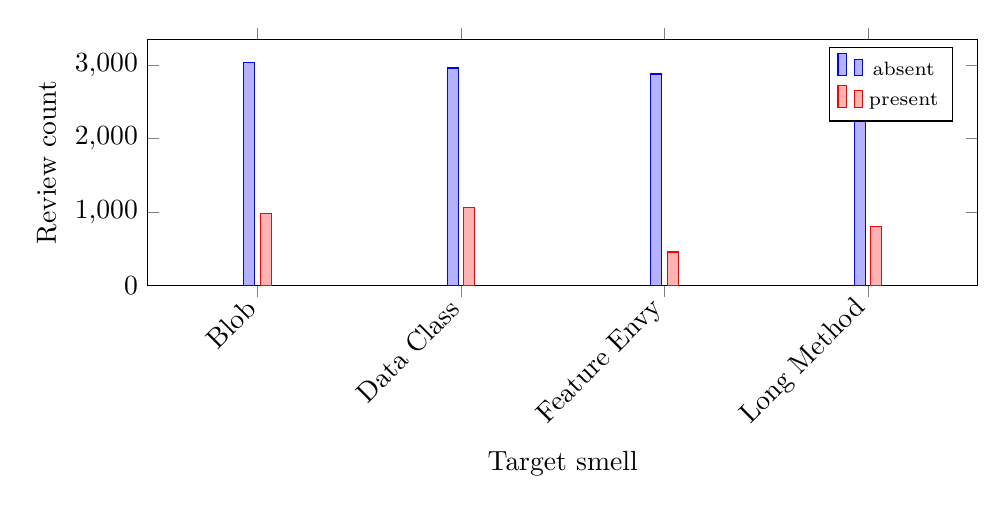
\begin{tikzpicture}
\begin{axis}[
    ybar,
    width=\columnwidth,
    height=4.7cm,
    bar width=4pt,
    ylabel={Review count},
    xlabel={Target smell},
    symbolic x coords={Blob,Data Class,Feature Envy,Long Method},
    xtick=data,
    x tick label style={rotate=45,anchor=east},
    ymin=0,
    legend style={at={(0.97,0.97)},anchor=north east,font=\scriptsize},
    enlarge x limits=0.18
]
\addplot coordinates {(Blob,3045) (Data Class,2964) (Feature Envy,2883) (Long Method,2556)};
\addplot coordinates {(Blob,974) (Data Class,1057) (Feature Envy,454) (Long Method,806)};
\legend{absent,present}
\end{axis}
\end{tikzpicture}
\caption{Review-level binary label distribution by code smell type.}
\label{fig:class-imbalance}
\end{figure}

\subsection{Data Preprocessing}
\label{subsec:data-preprocessing}

\subsubsection{Prompt Construction}

After retrieving the samples, we created a prompt for each review to use as the model input. The prompt asks the model to determine whether the sample contains the target smell type. It includes the smell type being evaluated, the source code associated with the sample, and the expected output format.

\subsubsection{Reviewer Disagreement}

After preprocessing, we had 8,711 unique sample-smell pairs, 1,007 of which had reviewer disagreement. This means that, for some sample-smell pairs, different reviewers assigned severities that were mapped to different binary labels.

To stay consistent with how the MLCQ dataset is normally used, and to make our results comparable with earlier research, we did not remove the samples with reviewer disagreement. Therefore, the dataset remained review-based instead of being reduced to one final label for each sample-smell pair.

The number of unique sample-smell pairs is greater than the number of samples because each sample could be reviewed with respect to up to two smell types.

\subsubsection{Train/Validation/Test Split and Leakage Prevention}

To avoid data leakage, we split the data by sample rather than by review. When splitting the data using a 70/15/15 ratio, we made sure that all reviews of the same sample were placed in the same split. This means that the same sample cannot appear in more than one of the training, validation, and test sets.

We ended up with 9,383, 2,034, and 2,027 reviews in the training, validation, and test splits, respectively. These add up to the full set of 13,444 usable reviews. We also recorded the label distribution and smell type distribution in each split (Table~\ref{tab:split-distribution}) to check that the split did not introduce major bias.

\begin{table}[t]
\caption{Train, validation, and test label distribution.}
\label{tab:split-distribution}
\centering
\begin{tabular}{lrrr}
\hline
Split & Reviews & Absent & Present \\
\hline
Train & 9,383 & 7,332 & 2,051 \\
Validation & 2,034 & 1,580 & 454 \\
Test & 2,027 & 1,565 & 462 \\
\hline
\end{tabular}
\end{table}

The cleaned dataset was then saved and used for training and evaluating the models.

\subsection{Model Training}
\label{subsec:model-training}

We used the same configurations and pipeline for training all models, with very few exceptions that are explicitly documented in this work. The training and optimization settings used across the experiments are summarized in Table~\ref{tab:training-config}. The binary classification setup and LoRA configuration are summarized in Table~\ref{tab:lora-config}.

The training of all models was done on a Tesla T4 GPU available on free Kaggle accounts.

\subsubsection{Model Selection}

The models trained in this work are:

\begin{itemize}
\item Qwen/Qwen3-0.6B
\item Qwen/Qwen3-1.7B
\item meta-llama/Llama-3.2-1B-Instruct
\item google/gemma-3-1b-it
\item deepseek-ai/DeepSeek-R1-Distill-Qwen-1.5B
\end{itemize}

All selected models are lightweight LLMs with fewer than 2B parameters.

\subsubsection{Class Weighting}
\label{subsubsec:class-weighting}

We first loaded the cleaned dataset that was saved after preprocessing. Then, we used only the training split to calculate the class weights.

The class weights were calculated using the formula:

\[
\text{class\_weight} = \frac{\text{total training examples}}{\text{number of classes} \times \text{class count}}
\]

where \texttt{number\_of\_classes} is 2, since the labels are absent and present, and \texttt{class\_count} is the number of training examples belonging to the class we are calculating the weight for.

These weights were then used in weighted cross entropy during training. We did this to reduce the effect of the class imbalance discussed earlier. Without using class weights, the model could mostly predict the majority class, which is absent, and still get a relatively high accuracy. The weights came out to around 0.64 for the absent class and 2.29 for the present class, which reflects the imbalance between the two labels.

\subsubsection{Tokenisation and Input Preparation}

Before training, the prompts were converted into token sequences using the tokenizer associated with each model. This was necessary because the selected models do not all use the same vocabulary or tokenisation scheme, so each prompt had to be represented in the format expected by the model being trained.

For consistency across all experiments, the maximum input length was set to 512 tokens. Prompts that exceeded this limit were truncated before being passed to the model.

Shorter inputs were padded during batching so that examples with different lengths could be processed together. Padding was applied at the batch level, while truncation was applied during tokenisation.

\subsubsection{Model Architecture and Parameter-Efficient Fine-Tuning}

Each selected model was adapted for binary sequence classification. Given an input prompt, the model outputs scores for two possible labels: absent and present.

Instead of fully fine-tuning all model parameters, we used LoRA as a parameter-efficient fine-tuning method. With this approach, most of the original model parameters remain frozen, and only a small number of additional trainable parameters are updated during training. This reduces the memory and computational cost of fine-tuning.

In our setup, LoRA was applied to the query and value projection modules in the attention layers. A classification head with two outputs was used to produce scores for the absent and present labels. For Qwen/Qwen3-0.6B, this resulted in 1,148,928 trainable parameters out of 597,200,896 total parameters, meaning that only 0.1924\% of the parameters were updated during training.

This setup allowed us to fine-tune all selected lightweight LLMs using the same general training pipeline while keeping the experiments feasible within the available computational resources.

\subsection{Evaluation Metrics}
\label{subsec:evaluation-metrics}

We calculated accuracy, precision, recall, and F1 score on the training, validation, and test sets, with the results reported per smell type. Since the dataset is imbalanced, we paid particular attention to the results for the present class. Insights from these results are discussed in Section~\ref{sec:results}.

The meaning and calculation of each metric are also provided in Table~\ref{tab:evaluation-metrics}.

\begin{table}[t]
\caption{Evaluation metrics and their calculations.}
\label{tab:evaluation-metrics}
\centering
\begin{tabular}{>{\raggedright\arraybackslash}p{0.24\linewidth}>{\raggedright\arraybackslash}p{0.63\linewidth}}
\hline
Metric & Calculation \\
\hline
Accuracy & $(TP + TN) / (TP + TN + FP + FN)$ \\
Precision & $TP / (TP + FP)$ \\
Recall & $TP / (TP + FN)$ \\
F1-score & $2 \times (\text{Precision} \times \text{Recall}) / (\text{Precision} + \text{Recall})$ \\
\hline
\end{tabular}
\end{table}
